\documentclass[12pt]{article}

\usepackage[margin=0.5in, includefoot]{geometry}
\usepackage{tikz}
    \newlength{\arrowsize}  % https://tex.stackexchange.com/questions/5461/is-it-possible-to-change-the-size-of-an-arrowhead-in-tikz-pgf/161238#161238
    \pgfarrowsdeclare{biggertip}{biggertip}{  
        \setlength{\arrowsize}{0.5pt}  
        \addtolength{\arrowsize}{.5\pgflinewidth}  
        \pgfarrowsrightextend{0}  
        \pgfarrowsleftextend{-5\arrowsize}  
    }{  
        \setlength{\arrowsize}{0.5pt}  
        \addtolength{\arrowsize}{.5\pgflinewidth}  
        \pgfpathmoveto{\pgfpoint{-5\arrowsize}{4\arrowsize}}  
        \pgfpathlineto{\pgfpointorigin}  
        \pgfpathlineto{\pgfpoint{-5\arrowsize}{-4\arrowsize}}  
        \pgfusepathqstroke  
    }  
\usepackage{setspace}
\usepackage{titlesec}
    \titleformat{\subsubsection}{\normalfont\normalsize\itshape}{\thesubsubsection}{1em}{}
\usepackage{hyperref}
\usepackage{xurl} % yay this works
    \hypersetup{
        colorlinks=true, 
        linkcolor=blue, % can comment this out if the blue figure faces is bothersome
        urlcolor=cyan
    }
    \renewcommand{\figureautorefname}{\textbf{Figure}} % decent fix but later should figure out how to make numbers bolded too
\usepackage{enumitem}
    \setlist[enumerate]{label=(\arabic*)}
\usepackage{amsmath}
\usepackage{amssymb} % for mathfrak font style
\usepackage{mathrsfs} % for mathscr font style
\usepackage{bm}
\usepackage{physics}
\usepackage{cancel}
\usepackage{xfrac}
\usepackage{array}
\usepackage{multicol}
\usepackage{float}
\usepackage[many]{tcolorbox}
    \definecolor{cellborder}{HTML}{CFCFCF}
    \definecolor{cellbackground}{HTML}{F7F7F7}
\usepackage{listings}
    \lstset{
        basicstyle=\scriptsize\ttfamily, % font style
        escapeinside={(*@}{@*)} % escape into LaTeX using (*@ and @*)
    }
\usepackage{subcaption}
\usepackage{wrapfig}
\usepackage{graphicx}
\usepackage{multirow}
\usepackage{csvsimple}
\usepackage[font=small]{caption}
\usepackage{xcolor} % for formatting purposes
\usepackage{lipsum} % for formatting purposes
% \usepackage[hang, flushmargin]{footmisc} % seeing if default setup is actually nice looking

\renewcommand{\thesubsection}{\arabic{subsection}}
\newcommand{\displayinline}[1]{\displaystyle#1\mathstrut}
\newcommand{\totder}[2][]{\frac{\mathrm{d}#1}{\mathrm{d}#2}} % needs amsmath package
\newcommand{\sectotder}[2][]{\frac{\mathrm{d^2}#1}{\mathrm{d}#2^2}}
\newcommand{\parder}[2][]{\frac{\mathrm{\partial#1}}{\mathrm{\partial#2}}} % needs amsmath package
\renewcommand{\Re}{\mathfrak{Re}} % these are just cooler
\renewcommand{\Im}{\mathfrak{Im}}
\newcommand{\im}{\mathrm{i}}
\newcommand{\diff}[1]{\text{d}#1}
\newcommand{\R}{\mathbb{R}}

\newsavebox\foobox
\newlength{\foodim}
\newcommand{\slantbox}[2][0]{\mbox{%
        \sbox{\foobox}{#2}%
        \foodim=#1\wd\foobox
        \hskip \wd\foobox
        \hskip -0.5\foodim
        \pdfsave
        \pdfsetmatrix{1 0 #1 1}%
        \llap{\usebox{\foobox}}%
        \pdfrestore
        \hskip 0.5\foodim
}}
\def\Lagrangian{\slantbox[-0.2]{$\mathcal{L}$}} % ok wow nailed it (I think?)
\def\Fourier{\slantbox[-0.45]{$\mathscr{F}$}} % kinda legible yeah

\newcommand{\mtauonea}{\mathrm{M\tau1}\text{-}\mathrm{A}}

\begin{document}
\setstretch{1.15}

\section*{Applications of Magnetic Torque to Various Static and Dynamic Experiments}

\begin{quote}
    Jeff Lam, Victoria Herrada \\
    \textit{Department of Physics, Binghamton University} \\
    May 4\textsuperscript{th}, 2025
\end{quote}

\subsection*{Abstract}
The $\mtauonea$ instrument designed by TeachSpin Inc. applies the concept of magnetic torque
across three possible experiments:
(1) \textit{Magnetic vs. Gravitational Torques};
(2) \textit{Harmonic Oscillation of a Spherical Pendulum};
and (3) \textit{Precessional Motion of a Spinning
Sphere}, where (1) is a form of static experiment and (2) \& (3) are forms of dynamic experiments.
In all cases, the magnetic dipole moment $\mu$ of a neodynium magnetic can be determined
through careful data collection on the strength of the generated external magnetic field,
applicable parameters when the experiment calls for them such as the housing cue ball's diameter,
mass of the cue ball, \textit{etc}., and timings of periodic motion for the dynamic experiments.
Linear least-squares fitting is applicable across all three experiments,
and for every model a predictive slope parameter $a$ can be calculated to help
derive experimental values of $\mu$ from theoretical relationships establised for each experiment.
These relationships were determined to be $a\propto\dfrac{mg}{\mu}$, $a\propto\dfrac{4\pi^2I}{\mu}$,
and $a\propto\dfrac{\mu}{L}$ for measurable values $B$, $T$, and $\Omega_p$ with respect to each experiment,
where $I$ is moment of inertia of a sphere, $L$ is large spin angular momentum of a rotating cue ball,
$T$ is oscillation period of the spherical pendulum, and $\Omega_p$ is precessional period of the spinning sphere.
For an accepted $\mu$ value of 0.4 $\mathrm{A\cdot m^2}$,
the experiments yielded values with percent errors of 4.5\%, 24.65\%, and 46.44\%.
The increasing percent error values likely is due to dismissal of small angle approximation
for the dynamic experiments when carried out.

\noindent\rule{\linewidth}{0.5pt}

\begin{multicols}{2}

\subsection{Introduction}
Electric motors capable of converting electrical energy to mechanical energy are the most common application involving torque---
in all cases, however, an external magnetic field is almost always necessary.
This is typically done via two ways when given a loop of current:
(1) using a split-ring commutator to essentially produce Alternating Currents (AC) if the external magnetic field is constant in one direction; 
or (2) producing AC magnetic fields if given a Direct Current (DC) loop (typically then the magnetic field is supplied by AC coils as electromagnets).
Nevertheless, the torque produced by these scenarios
\begin{figure}[H]
    \centering
    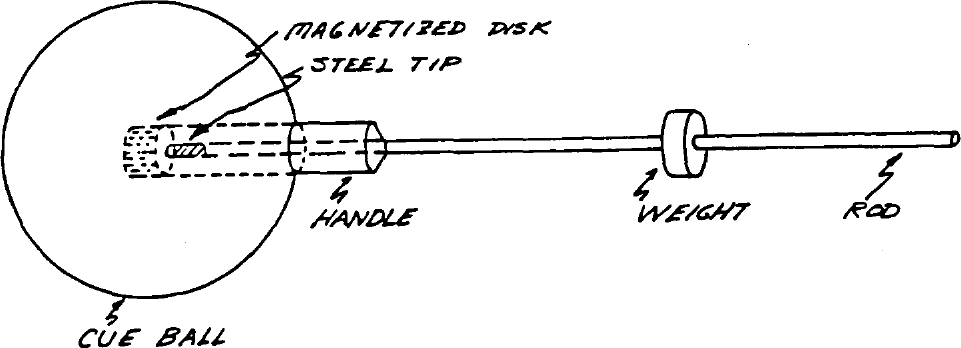
\includegraphics[width=0.98\linewidth]{figs/fig1.png}
    \caption{Schematic diagram of $\mtauonea$'s cue ball.}
\end{figure}
\noindent
is due to an external magnetic field and the loop of wire acting as a magnetic dipole.

While the experiments outlined by this paper essentially only apply magnetic torque for a single moment (\textit{i.e.}, no AC applications for continuous rotation),
there are rich static and dynamic procedures that can be followed to experimentally determine a magnetic dipole moment within an external magnetic field.
In this paper, the theory and laboratory procedures of three experiments were explored:
\begin{itemize}
    \item[] \textit{Part I: Magnetic vs. Gravitational Torques}
    \item[] \textit{Part II: Harmonic Oscillation of a Spherical Pendulum}
    \item[] \textit{Part III: Precessional Motion of a Spinning Sphere}
\end{itemize}

\subsection{Setup Specifications}
All experiments were designed by TeachSpin Inc., and furthermore,
the instrument used to carry out these experiments was also provided by them.
This instrument is referred by TeachSpin as ``MAGNETIC TORQUE $\mtauonea$''---
in this paper it is simply referred to as $\mtauonea$.
Provided by the kit are a few specially tailored parts.

\subsubsection{The Cue Ball}
\textbf{Figure 1} is a provided schematic diagram of what TeachSpin dubs the ``cue ball'' for their $\mtauonea$,
along with other specifications in which the majority were used in \textit{Part I} of the experiments.
As it can be seen, the core of the cue ball houses a magnetized disk,
specifically a $\mathrm{Nd_2Fe_{14}B}$ (neodynium iron boron) permanent magnet,
\textit{a.k.a.} a neodynium magnet, which initially seems to contradict the
introduction of magnetic torque as usually involving a loop of current as the
magnetic dipole.
However, TeachSpin assures that the permanent magnet is magnetized such that the
magnetic field produced is along the axis of the handle as shown in the figure,
acting as if it was an ideal magnetic dipole.

\subsubsection{M$\tau$1-A}
The overall objective across all three experiments designed by TeachSpin
is to experimentally derive
\begin{figure}[H]
    \centering
    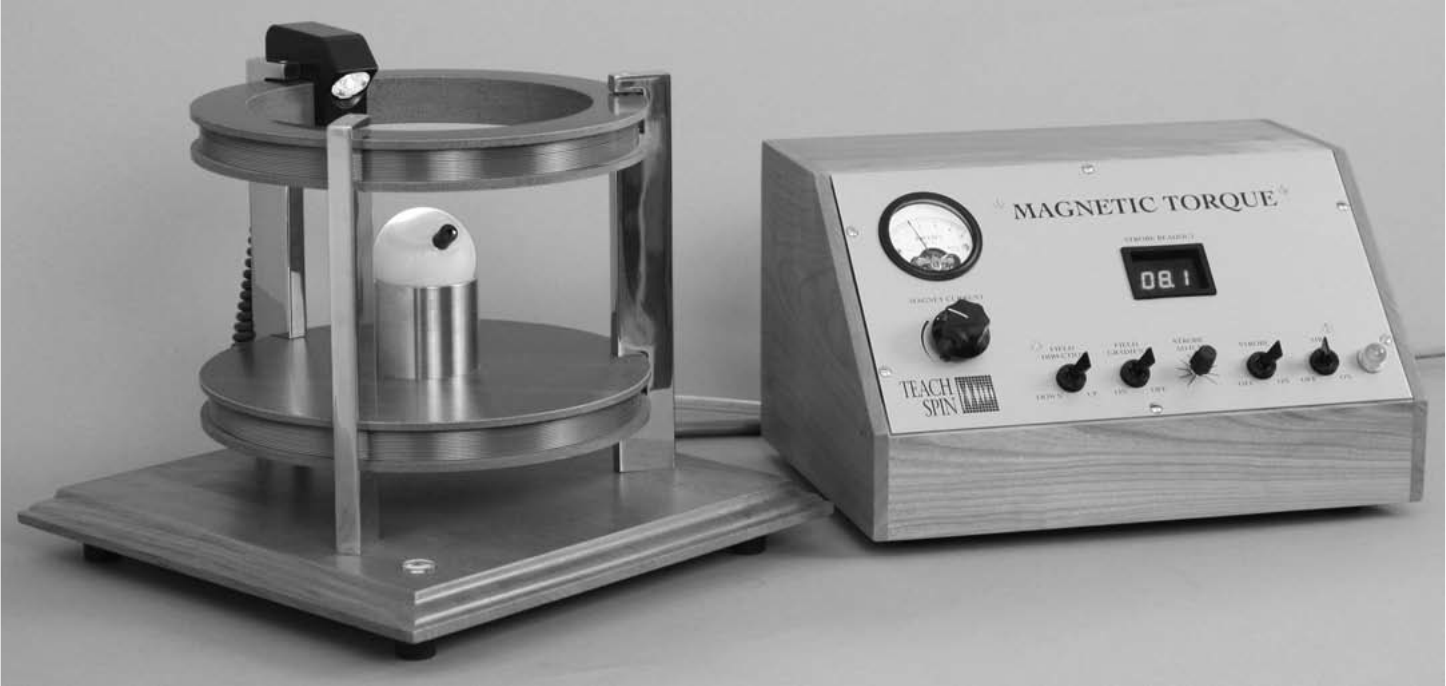
\includegraphics[width=0.98\linewidth]{figs/fig2.png}
    \caption{
        Provided image from a brochure titled ``Magnetic Torque: A `Classic' Made Even Better'',
        featuring $\mtauonea$. More features of $\mtauonea$ can be seen as a set of Helmholtz coils,
        an air bearing, a strobe light, and a control box to tune every one of them [\hyperref[sec:1]{1}].
        }
\end{figure}
\noindent
a value for the magnetic dipole moment of the neodynium
magnet from various applications of magnetic torque.
\textbf{Figure 2} provides a photograph showcasing the rest of the $\mtauonea$ instrument.
According to the included reference as well, $\mtauonea$ comes with a pair of Helmholtz coils
made out of 195 turns of \#18 copper wires, an air bearing at the center which is also
specifically designed such that the cue ball is raised to house the neodynium magnet at the
center of the coils, a strobe light for assistance in carrying out experiment \textit{Part III},
and a control box which also houses an air pump and power supply for the platform.
Some important notes of these specifications is that the Helmholtz coils help produce a uniform magnetic
fields [\hyperref[sec:2]{2}] and the air bearing helps ensure minimum friction between the cue ball and bearing socket---
an observer may then assume it being negligible across all experiments.

Some things to note from the specifications provided by the reference is first a detail that
the \textit{magnetic moment of the magnetized disk should measure as 0.4 $A\cdot m^2$}---
this value act as the accepted answer across all experiments done in this paper.
From both the included reference and the $\mtauonea$ lab manual,
the magnetic field supplied by the Helmholtz coils were appreciably calculated by
TeachSpin as $B=1.36\pm0.03\times10^{-3}$ T/A---
these values assist in determining the strength of the $B$ field for a given current reading
throughout section \textbf{4 Methods and Data Analysis}
(and the uncertainty values were especially used for the least-squares fitting for \textit{Part I} of the experiments).

\subsection{Theory}

\subsubsection{The Theory Behind Part I}
\textbf{Figure 3} helps demonstrate the theoretical setup for balancing magnetic and gravitational torques.
In many introductory physics II curriculums, it can be shown that for a magnetic moment $\mu$ within an external
magnetic field $B$, the torque produced by the misalignment of the two vectors can be evaluated via the cross 
product $\tau=\mu\times B$, where $\tau$ is a pseudovector representing torque.
Because the definition involves the cross product,
the direction of $\tau$ can be determined via the right-hand rule---
curling one's fingers starting from the vector representing $\mu$ to the vector representing $B$.
The right-hand rule is also the reason why torque due to a magnetic dipole moment $\tau_B$
is a vector pointing outside of the page, as confirmed by the figure.

If one were to attached the aluminum rod (assumed to be massless) and furthermore attach the disk carrying a mass $m$
at a distance $r$ away from the cue ball's center of mass, a second torque would be produced due to gravity.
The formula for the torque produced by this setup can also be derived from any typical introductory physics I curriculum,
given as $\tau=r\times mg$. The right-hand rule may also be used in this scenario to determine the direction of $\tau_g$
the torque due to gravity as pointing inside of the page--- this is also confirmed by the figure.

Because $\tau_B$ and $\tau_g$ points opposite to each other, Newton's First Law of Motion
for rotational kinematics may be applied if the system is setup such that no net torque acts on the system,
\textit{i.e.}, $\tau_B=\tau_g$. From there it can be shown that
$$\mu\times B = r\times mg\longrightarrow\mu B\sin(\theta)=rmg\sin(\theta)$$
\begin{figure}[H]
    \centering
    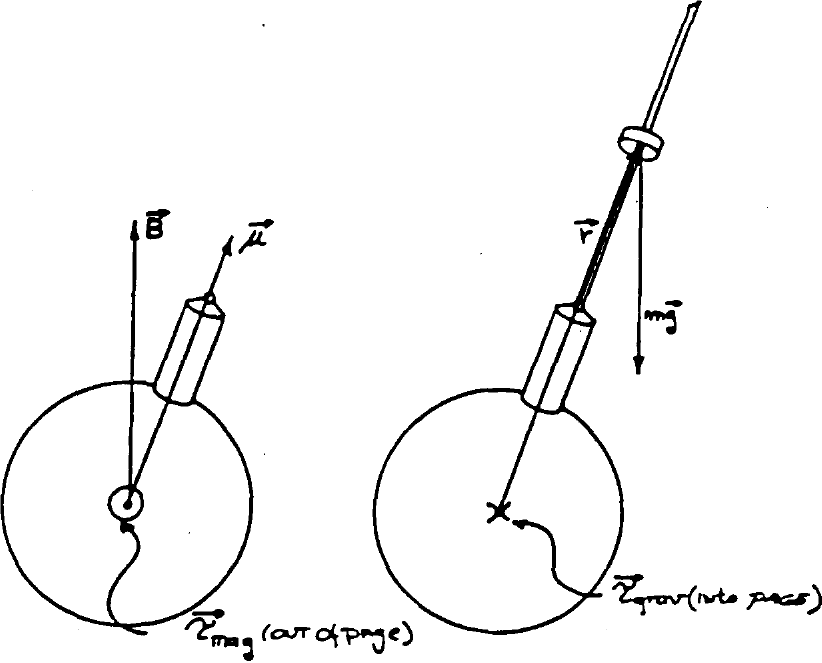
\includegraphics[width=0.98\linewidth]{figs/fig3.png}
    \caption{
        Schematic setup of the theory behind balancing magnetic and gravitational torques
        from the $\mtauonea$'s manual.
    }
\end{figure}
\noindent
where $\theta$ represents the angle spanned from the cross product of either side.
Choose the balance of the system to be when the aluminum rod is horizontal. Then $\theta=\frac{\pi}{2}\rightarrow\sin\qty(\frac{\pi}{2})=1$.
From this relationship, one may derive a formula for $B$ as $B=\dfrac{mg}{\mu}r$,
allowing one to derive an experimental linear slope from a least-squares fitting to derive a value for $\mu$.
It is worth noting that the relationship derived in this step departures from what was provided from
$\mtauonea$'s lab manual (where it was instead derived as $r=\dfrac{\mu}{mg}B$),
for a different experimental procedure was followed when gathering data.

\subsubsection{The Theory Behind Part II}
Because this and \textit{Part III} of the experiments are dynamics,
Newton's Second Law of Motion for rotational kinematics may be applied.
Take Newton's Second Law in the form of $\displaystyle\sum\tau=\totder[L]{t}$,
analagous to force being the time derivative of momentum in translational kinematics.
It was already provided that the torque $\tau$ due to a uniform magnetic field can be expressed as $\mu\times B$. 
However, consider the scenario again where $\mu$ is misaligned with the external magnetic field $B$:
the torque produced from the misalignment will act such that it would move \textit{against}
the angular displacement of $\mu$, \textit{i.e.}, the torque is a \textit{restorative} torque,
analagous to how spring force is a restorative force in translational kinematics.
Then Newton's Second Law in this scenario may be expressed as
$$-\mu\times B=\totder[L]{t}$$
Use the definition of cross product on the left-hand side and the definitions
$L=I\omega$ and $\displaystyle \omega=\totder[\theta]{t}$ on the right-hand side
to further express the differential equation as
$$-\mu B\sin(\theta)=I\sectotder[\theta]{t}$$
Take $\sin(\theta)\approx\theta$ for small angular displacements between the dipole moment and the direction of the
uniform magnetic field. Then the expression $\displaystyle -\mu B\theta=I\sectotder[\theta]{t}$ may be solved as simple
harmonic motion:
$$\theta(t)=A\cos(\omega t)$$
where $\omega=\sqrt{\dfrac{\mu}{I}B}$. If one were to instead measure periods of oscillation rather than angular frequency,
then the definitions $\omega=2\pi\nu$, $\nu=\dfrac{1}{T}$ closes a form of the period for the cue ball acting as a spherical
pendulum moving under simple harmonic motion as
$$T^2=\frac{4\pi^2I}{\mu}\frac{1}{B}$$
where in this scenario, moment of inertia $I$ is taken as $\frac{2}{5}mr^2$ for the mass $m$ and spherical radius $r$ of the cue ball.
Similarly to experiment \textit{Part I}, a linear least-squares fitting model can help produce an experimental slope value to determine $\mu$.

\subsubsection{ The Theory Behind Part III}
Precession is defined as the change in orientation of a rotating body's axis of rotation.
Precession in fact occurs within Earth's rotation, in which its effect manifests as the reason why
some seasons are more
\begin{figure}[H]
    \centering
    \begin{tikzpicture}
        \draw[-biggertip] (0,-3) -- (0,0);
        \draw[-biggertip] (0,0) -- (3,0);
        \draw[-biggertip] (0,-3) -- (3,0);
        \draw[domain=45:90] plot ({cos(\x)}, {sin(\x)-3});
        \draw node at (-0.3, -1.3) {$B$};
        \draw node at (1.5, 0.3) {$L\sin(\theta)$};
        \draw node at (1.9, -1.6) {$L$};
        \draw node at (0.5, -1.8) {$\theta$};
        \draw node at (1.5, -4.1) {\small(a)};

        \draw[-biggertip] (4,-3) -- (7,-3);
        \draw[-biggertip] (4,-3) -- (6.718923361, -1.732145215); % this is at 25 degrees
        \draw[-biggertip] (7,-3) -- (6.718923361, -1.732145215);
        \draw[domain=0:25] plot ({cos(\x)+4}, {sin(\x)-3});
        \draw node at (5.6, -3.4) {$L\sin(\theta)$};
        \draw node at (5, -1.8) {$L\sin(\theta)'$};
        \draw node at (7.3, -2.3) {$\Delta L$};
        \draw node at (5.5, -2.7) {$\Delta\phi$};
        \draw node at (5.5, -4.1) {\small(b)};
    \end{tikzpicture}
    \caption{
        Trigonometric relationships for proving precessional angular velocity
        as $\Omega_p=\dfrac{\mu}{L}B$. (a) represents a side view of the spinning
        tilted cue ball, where $L$ points at the same direction as the axis tilt,
        and (b) represents a top view of when the large spin angular momentum $L$
        changes due to a weak torque.
    }
\end{figure}
\noindent
extreme in one hemisphere than another [\hyperref[sec:3]{3}].

Start with the result of applying Newton's Second Law from the last section, $\displaystyle \mu\times B=\totder[L]{t}$,
but this time $L$ represents the spin angular momentum of the rotating body (\textit{i.e.}, the cue ball spinning).
\textbf{Figure 4} will help visualize how precession motion arises.
From \textbf{4a}, it can be seen that $L$ points in the same direction as the axis tilt---
to measure the precessional angular displacement, a top arrow representing $L\sin(\theta)$ is drawn.
The transition to \textbf{4b}, a top view of the rotating object now, showcases how a small change in angular momentum
$\Delta L$ is caused by a small change in precessional angular displacement $\Delta\phi$ due to a weak torque [\hyperref[sec:4]{4}].
Since these changes are small, the resultant vector can be well-approximated as an arc via the formula $s=r\phi$.
Then the change in spin angular momentum can be expressed as $\Delta L=\Delta\phi L\sin(\theta)$.
Take this over a small change in time $\Delta t$ and take the limit as $\Delta t$ approaches to zero:
$$\lim_{\Delta t\to0}\frac{\Delta L}{\Delta t}=\frac{\Delta\phi}{\Delta t}L\sin(\theta)$$
It is now appropriate to substitute these definitions in differential form. Then the change in angular momentum
over time is precisely
$$\totder[L]{t}=\Omega_p L\sin(\theta)$$
where $\Omega_p$ is the precessional angular velocity.

Take again the definition of cross product on the left-hand side of the result of Newton's Second Law,
and substitute the definition of $\displaystyle \totder[L]{t}$. It can be further simplified to
$$\mu B\sin(\theta)=\Omega_pL\sin(\theta)\;\longrightarrow\;\mu B=\Omega_pL$$
where the mutual $\sin(\theta)$ terms on either side cancel each other out.
Finally, a derivable relationship for $\Omega_p$ can be given as $\Omega_p=\dfrac{\mu}{L}B$.
Once again, a linear least-squares fitting model on an appropriately gathered data set will yield a slope term
to express a value for $\mu$

\subsection{Methods and Data Analysis}
All data gathered can be viewed in \textbf{Appendix A: Data Gathered Across All Experiments}.

\subsubsection{Magnetic vs Gravitational Torques}
This is \textit{Part I} of the experiments designed by TeachSpin.
The mass of the attachable disk $m$ was weighed in as 1.367 g and the diameter of the cue ball was
measured as 5.334 cm using a caliper (so the radius is measured as 2.667 cm).
Additionally, the length of the handle was measured as 1.25 cm using a preceision ruler\textsuperscript{$\dagger$}.
\renewcommand{\thefootnote}{$\dagger$}
\footnotetext{
    \textit{Note:} measuring the handle in the laboratory was a bit tricky since the cue ball is a bulky object itself,
    and most rulers do not start measuring from their end--- the measurement was taken \textit{with perspective} to correctly
    offset the ruler's starting measures.
}
The aluminum rod as shown before in \textbf{Figure 1} was plugged into the handle,
and in the same figure it can be seen that some of the rod's length gets embedded.
Using a marker, an initial tick was marked at where the handle ends on the rod,
then various 1 cm ticks were marked from that point towards the other end of the rod.
In total, eight 1 cm tick markers were introduced, but as it
\begin{figure}[H]
    \centering
    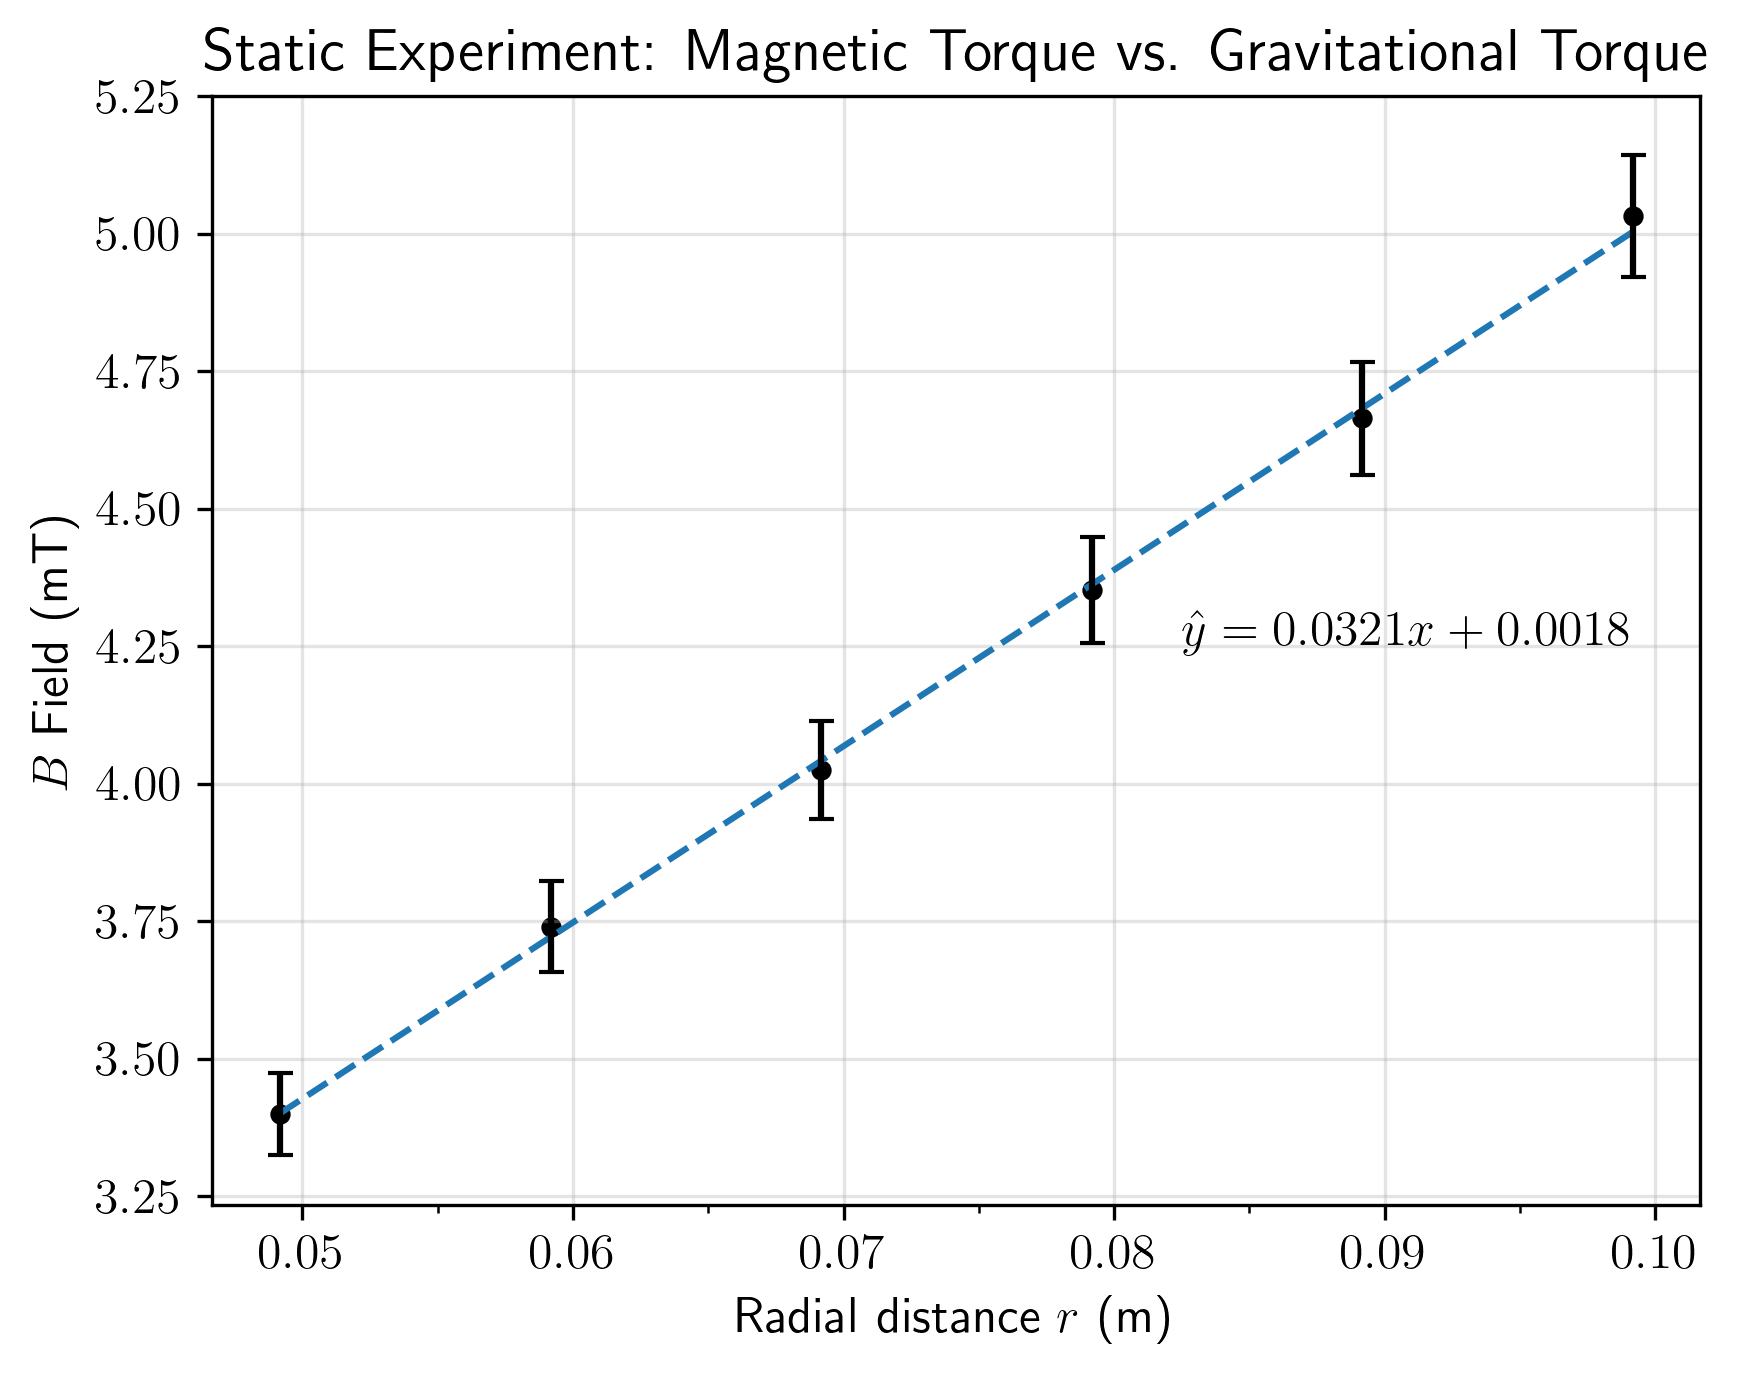
\includegraphics[width=0.98\linewidth]{figs/graph1.png}
    \caption{
        Scatterplot of experiment \textit{Part I: Magnetic vs. Gravitational Torques}.
        Error bars represent the uncertainty of the $B$ field supplied by the Helmholtz coils
        scaled by the amount of current flowing through the system.
        Uncertainties in the predictive parameters $a$, $b$ were significantly low that they are
        not shown in the graph.
    }
\end{figure}
\noindent
can be seen in \textbf{Appendix A},
the existence of only six rows in \textbf{Table 1} implies only data for the first six tick markers
could be collected. When the attachable disk was set on the first two markers from the rod's farthest end,
not even the maximum current $i$ that could be supplied (4 A) could create enough torque to counteract the 
gravitational torque due to the disk's weight (\textit{i.e.}, it was only at the 6 cm mark did the attachments lift).

The general procedure for gathering data follows by starting the air pump and turning on the magnetic field in the ``UP'' direction.
For every tick marker, the current supplying the Helmholtz coils were ``tuned'' via the current knob beneath the ammeter as shown in \textbf{Figure 2}
until the attached aluminum rod and disk lifts to a horizontal position.
During the process, the system may oscillate--- in these scenarios an observer temporarily held the system to help stabilize it from the motion before further tuning.
Once an appreciable horizontal position of the rod and disk was achieved,
the ammeter reading was recorded.
The ammeter of $\mtauonea$ has major ticks for every 1 A and minor tick markers for every 0.5 A---
the needle whenever it was between the ticks was approximated as some in-between value for recording.
Between each trial for each tick marker, the Helmholtz coils were monitored for their temperatures,
as hot coils could affect the readings from a weaker magnetic field.

\textbf{Figure 5} shows the data gathered for \textit{Part I} of the experiment graphed alongside its least-squares fitting.
The tick markers measuring in 1 cm, 2 cm, $\ldots$, 6 cm had the radius of the cue ball and the
length of the handle added to achieve the total radial distance $r$ from the center of masses between the cue ball and attachable disk.
The strength of the $B$ field for each current reading was determined using the value introduced from section \textit{2.2 M$\tau$1-A}.
For this experiment only, a weighted least-squares fitting model using the uncertainty of the $B$ field per Amp of current value given.
For the predictive slope parameter $a$, $a\propto\dfrac{mg}{\mu}$, and by substituing the appropriate values
$\mu$ for this experiment was approximated as 0.418 $\mathrm{A\cdot m^2}$.
The results of this experiment remarkably yielded a percent error of 4.5\% only,
which demonstrates the straightforward yet robust method of this experiment regarding measuring the value of $\mu$.
However, as it will be shown soon, the same cannot be said for the other parts of the experiment.

\subsubsection{Harmonic Oscillation of a Spherical
Pendulum}
For this part of the experiment, the only measurable value that needed to be determined was the weight of the cue ball.
The mass of the cue ball $m$ was measured to be 0.142 kg using a scale.
Like with the previous experiment, the air pump and Helmholtz coils were turned on,
starting with a current supply of 0.5 A.
With the cue ball sitting in the air bearing,
the handle was given an initial angular displacement before letting go,
setting the object off to simple harmonic motion.
20 oscillations of the motion was
\begin{figure}[H]
    \centering
    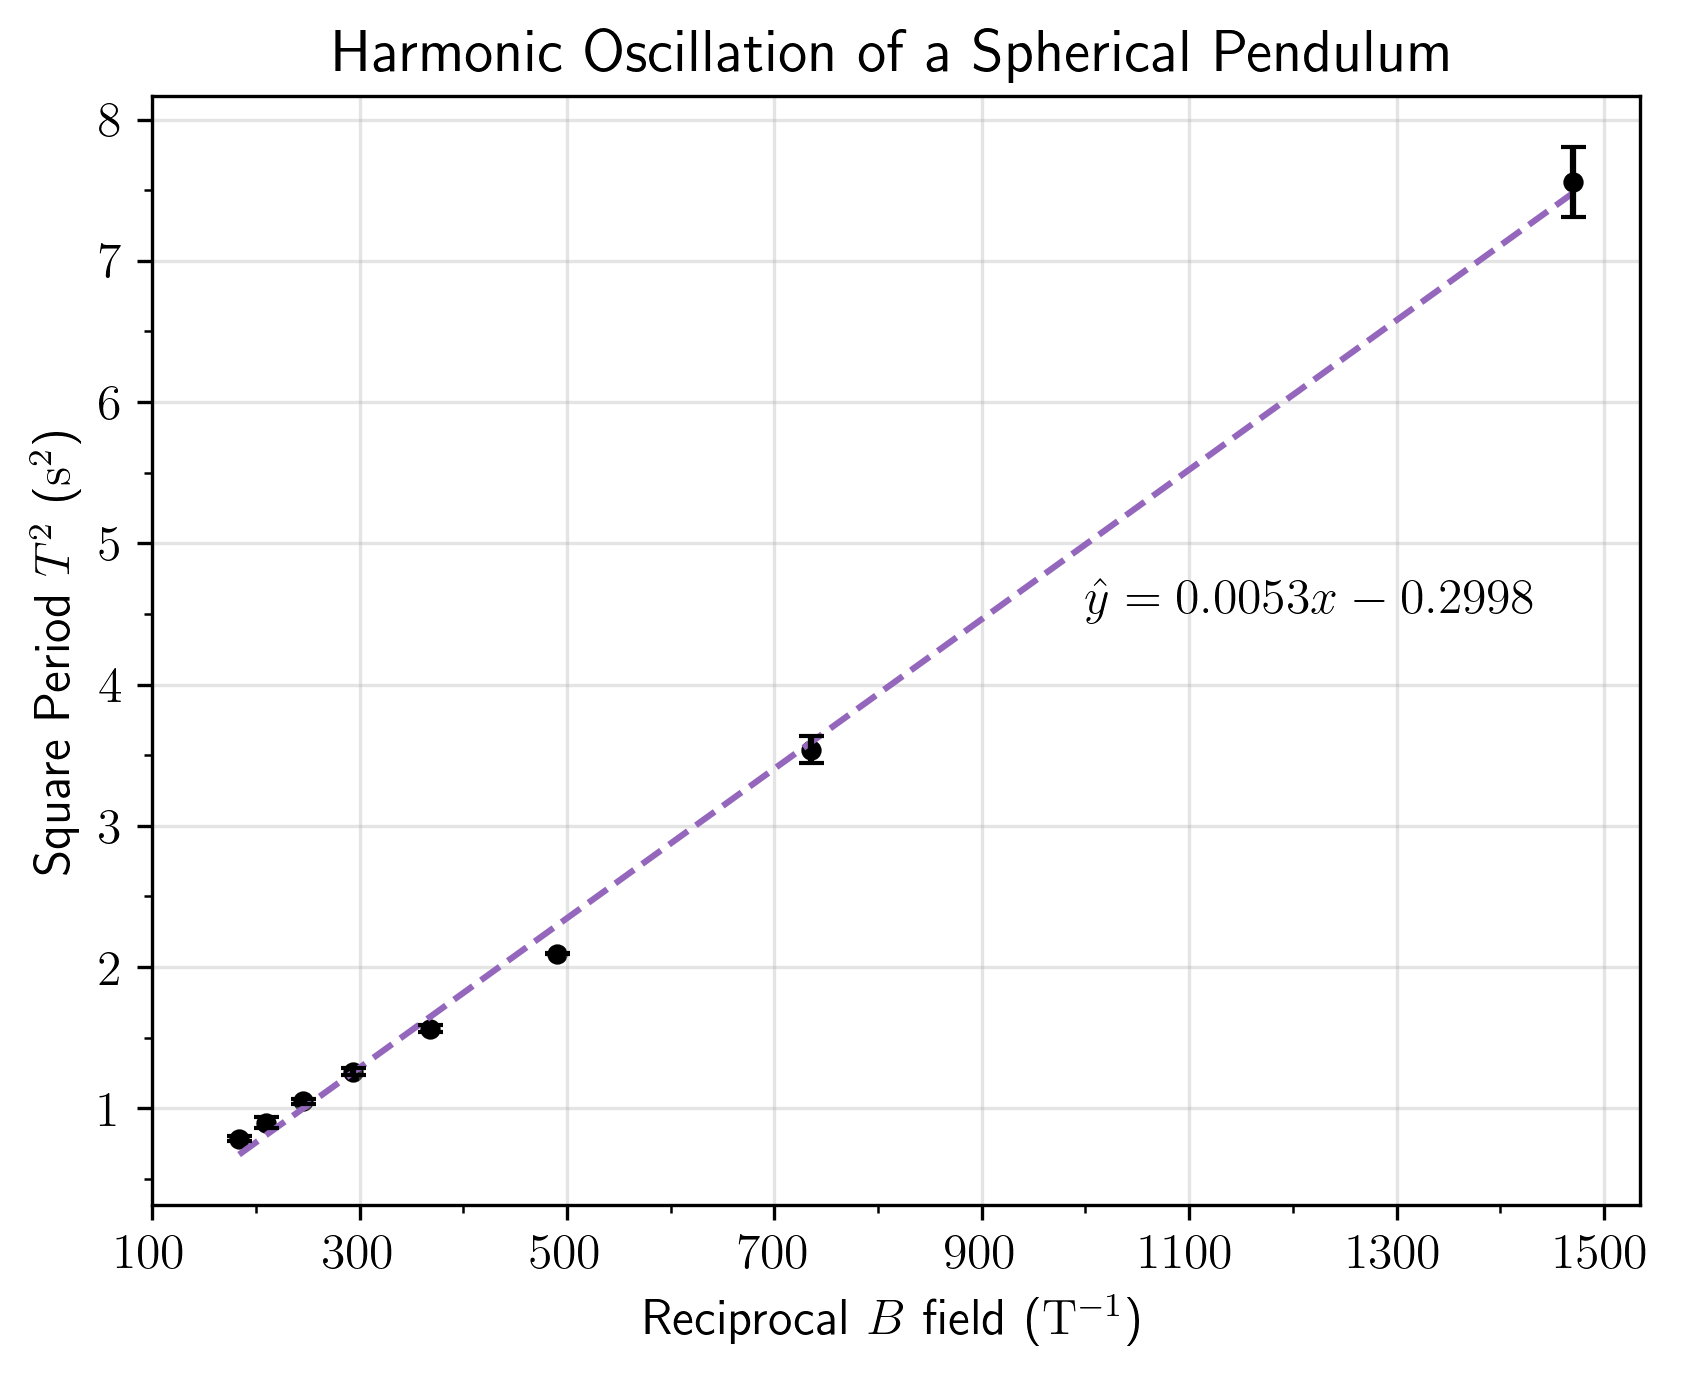
\includegraphics[width=0.98\linewidth]{figs/graph2.png}
    \caption{
        Scatterplot of experiment \textit{Part II: Harmonic Oscillation of a Spherical
        Pendulum}. Error bars represent the standard deviation of the three trials carried out for each
        oscillation timing of a given current reading.
        Like with \textit{Part I} of the experiments,
        uncertainties in the predictive parameters $a$, $b$ were
        significantly low, hence they are not reported.
    }
\end{figure}
\noindent
timed before repeating the procedure for the next 0.5 A reading,
up to the maximum 4 A that can be supplied. 
A total of three trials were carried out to account for variation in the least-squares fitting model.

\textbf{Figure 6} shows the data gathered for \textit{Part II} of the experiment graphed alongside its least-squares fitting.
The timing data was first converted to period of oscillations by simply dividing 20 for the count of oscillation observed,
then \textit{squared} since the relationship determined in section \textit{3.3 The Theory Behind Part II}
was determined as $T^2=\dfrac{4\pi^2I}{\mu}\dfrac{1}{B}$.
Similarly as the relationship is shown here, the \textit{reciprocal} of the $B$ field readings
were taken to properly allow the predictive slope parameter $a$ in the experiment to represent the grouped term being shown.
For the predictive slope parameter $a$, $a\propto\dfrac{4\pi^2I}{\mu}$.
As mentioned in the section \textit{3.3}, moment of inertia of the object can be calculated
by assuming the cue ball to be a sphere with uniform mass density, $I=\frac{2}{5}mr^2$.
The mass value and the radius value determined in the previous section was used as appropriate substitutions
to approximate the value of $\mu$ as 0.301 $\mathrm{A\cdot m^2}$.
Unlike the near precise experimentally determined value of $\mu$ in the previous section,
the $\mu$ value determined here suffers about a 24.65\% error.

\subsubsection{Precessional Motion of a Spinning Sphere}
No additional measurable value were needed for \textit{Part III} of the experiments.
The air pump of $\mtauonea$ was turned on, but this time \textit{no current was supplied yet}---
a measurable large spin angular frequency must first be set to cue ball alongside a tilt.
It has not been mentioned so far that near the hole of the handle where the attachable rod can be plugged in
is there a reflective white dot.
The use of the white dot and the strobe light helped set the cue ball in a tilted spin frequency of a known value.
And so, the lights of the laboratory was turned off,
and the strobe light was turned on, setting it at a value of 4.5 Hz.
The cue ball sitting on the air bearing was given a large body spin---
multiple attempts and resets were necessary for a bad spin could make
the object wobble.

When a stable spin was achieved, an observer would use \textit{the tip of their finger}
to help guide the spinning end of the handle to face the direction of the strobe light---
this also tilted the rotating object at approximately $45^\circ$.
With the lights out and strobe light on, the spin frequency of the cue ball can be viewed
as a form of stop-motion effect.
It can be intuitively understood that if the white dot on the handle is visible to the observer at one spot,
then the cue ball is spinning at the same frequency as the strobe light.
Likely, when initially viewing the white dot under the strobe light,
it is appearing across multiple places on the end of the handle.

An observer would wait until the white dot seemingly settle at a point before quickly
turning on the magnetic field to a starting current of 1 A
(quickly because the frequency of the ball's spin \textit{does change}
\begin{figure}[H]
    \centering
    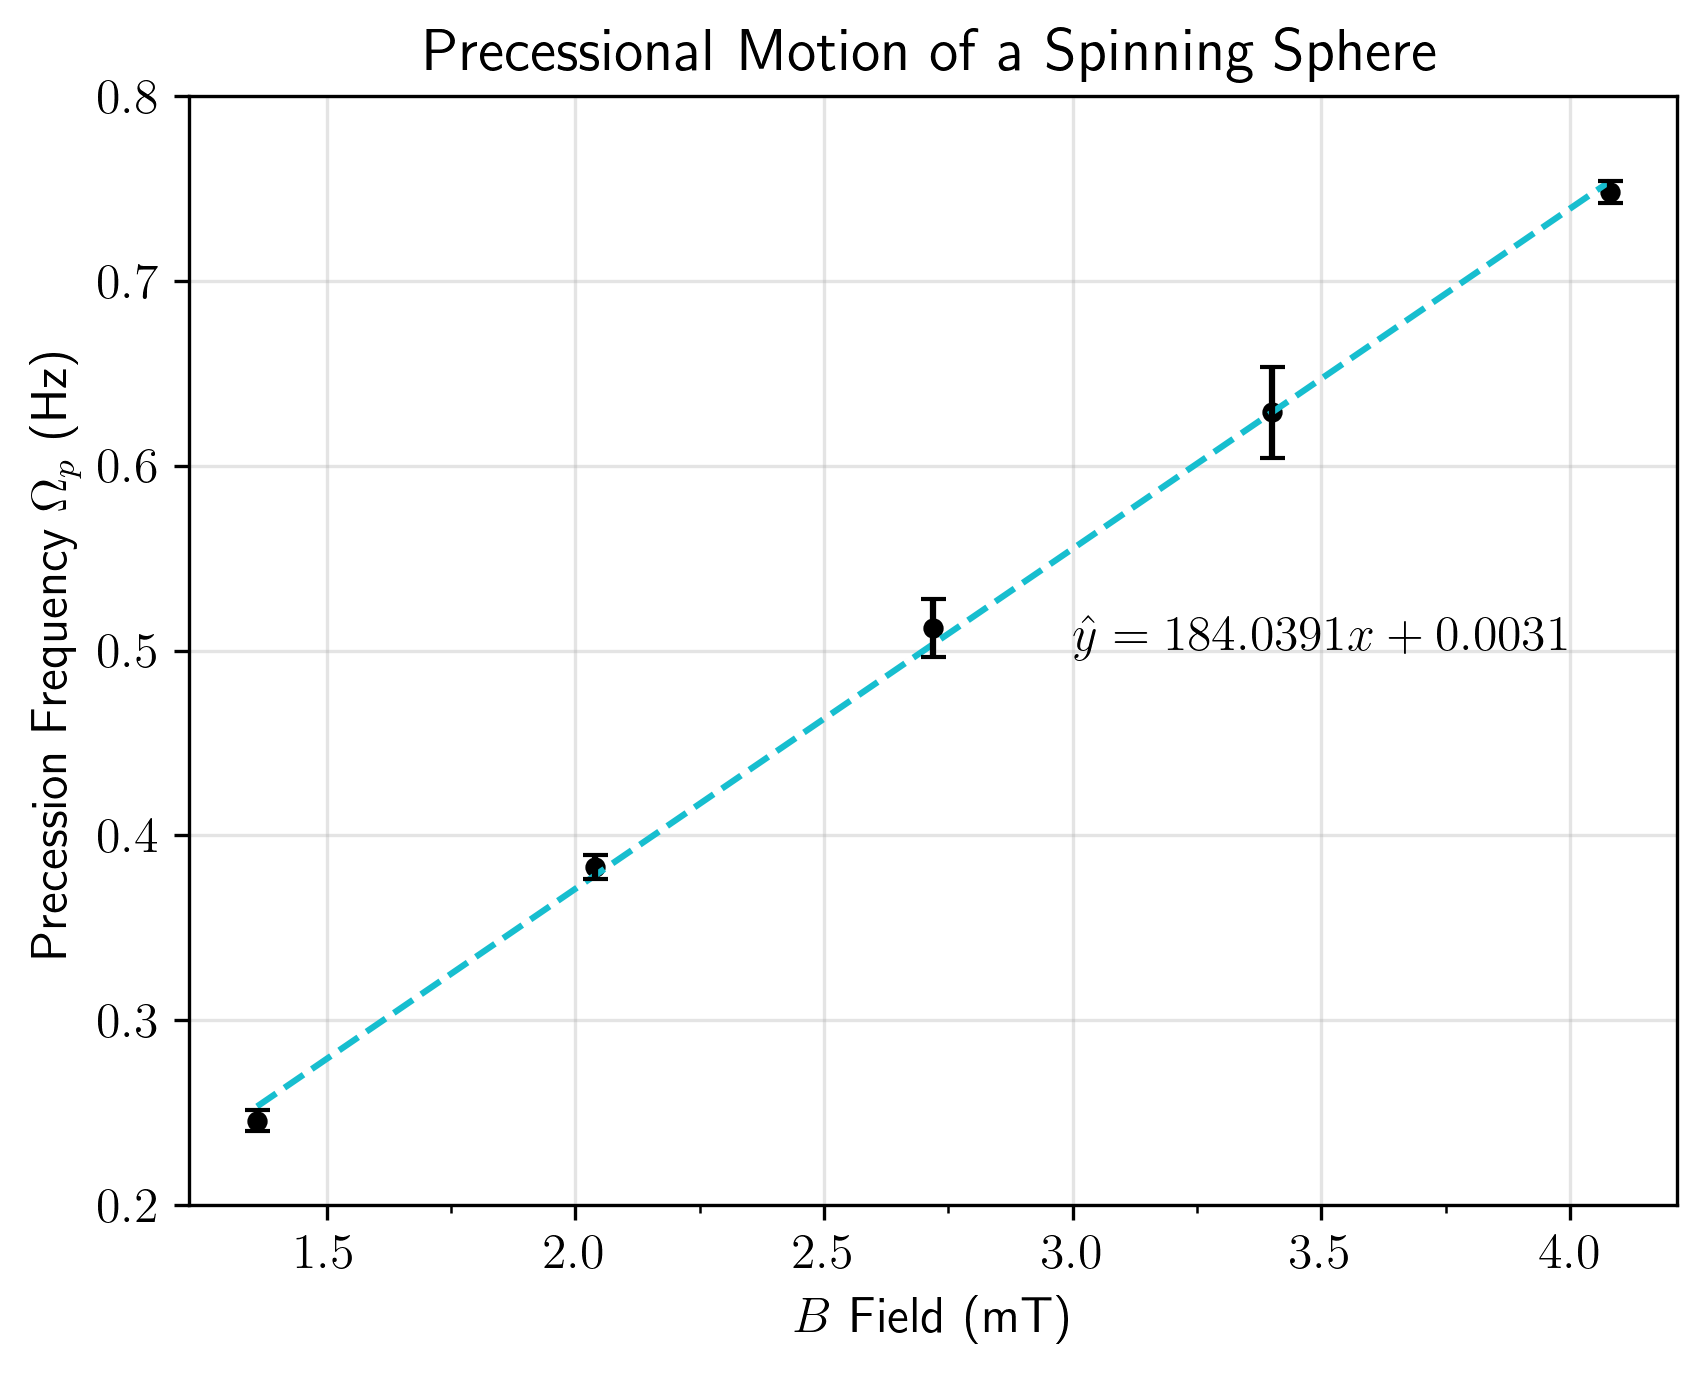
\includegraphics[width=0.98\linewidth]{figs/graph3.png}
    \caption{
        Scatterplot of experiment \textit{Part III: Precessional Motion of a Spinning
        Sphere}. Error bars represent the standard deviation of the three trials carried
        our for each one precessional period timing of a given current reading.
        Unlike the other least-squares fitting models, uncertainties found here are no longer significantly low
        such that they can be neglected: the uncertainty values for the parameters $a$, $b$
        were $\pm3.708$ T and $\pm0.011$ T, respectively, reported in the form of standard error.
    }
\end{figure}
\noindent
\textit{over time}, as a form of exponential decay).
After carefully tuning the magnetic field to the desired current supply,
the observer quickly looks back at the cue ball and times how long it takes for the object to do \textit{one} precession
around where the handle was first seen oriented.
Afterwards, the current was turned off and the cue ball was set at rest for the next measurement.
This procedure was repeated for the next 0.5 A readings, up to ideally the maximum 4 A that $\mtauonea$ can supply,
however data could only be gathered up to 3 A for further attempts in measuring precession period at current readings
higher than this introduced strong \textit{nutations} to the rotating object,
making it more difficult and therefore unrealiable to time its precession period.
Like with \textit{Part II} of the experiment, three trials were carried out
to account for variation in the least-squares fitting model.

\textbf{Figure 7} shows the data gathered for \textit{Part III} of the experiment graphed alongside its least-squares fitting.
The precessional period data can be converted to precessional frequency in Hz via dividing $2\pi$ with each
data point (a similar conversion was used in section \textit{3.2 The Theory Behind Part II}).
And like \textit{Part I} of the experiment, the current readings where each data point were gathered
can be converted to $B$ field strength using the value introduced in section \textit{2.2 M$\tau$1-A}.
For the predictive slope parameter $a$, $a\propto\dfrac{\mu}{L}$. The large spin angular momentum $L$
can be calculated using the definition $L=I\omega$, where $I$ is the moment of inertia of the cue ball
calculated previously and $\omega$ is angular frequency determined via simply multiplying $2\pi$ to 4.5 Hz.
The results of the experiment yielded a $\mu$ value of 0.210 $\mathrm{A\cdot m^2}$,
a significantly worse result than what was concluded in \textit{Part II} of the experiments,
suffering a percent error of 47.44\%.

\subsection{Conclusion}
Overall, the $\mtauonea$ instrument designed by TeachSpin introduces exciting experiments
to explore various applications of magnetic torque. Out of the three experiments designed by
them, the first one seemed straightforward enough that it yielded correct results,
while the other two can be considered significantly harder to do the same.
Likely avenues of errors introduced that could explain how the $\mu$ values begin
to differ are for \textit{Part II} of the experiments, too large of an angular
displacement was set for every reading (very similarly to the Coupled Pendulums Experiment),
and for \textit{Part III} of the experiments, a similar conclusion follows:
too large of a tilt angle likely interfered with the precession and may even likely
be the cause behind the nutation at current readings greater than 3 A.

\end{multicols}

\newpage
\subsection*{References}
\begin{enumerate}[label={[\arabic*]}]
    \item \label{sec:1} Magnetic Torque, \textit{TeachSpin, Inc.}, \url{https://www.teachspin.com/magnetic-torque}
    \item \label{sec:2} Richtberg, Stefan. Magnetic field of two Helmholtz coils, \textit{Ludwig Maximilian University of Munich}, \url{https://virtuelle-experimente.de/en/b-feld/b-feld/helmholtzspulenpaar.php}
    \item \label{sec:3} NASA Science Editorial Team, Milankovitch (Orbital) Cycles and Their Role in Earth's Climate, \textit{NASA}, \url{https://science.nasa.gov/science-research/earth-science/milankovitch-orbital-cycles-and-their-role-in-earths-climate/}
    \item \label{sec:4} Taylor, John R. \textit{Classical Mechanics} (University Science Books, 2003), p. 392
\end{enumerate}

\newpage
\subsection*{Appendix A: Data Gathered Across All Experiments}

\begin{table}[H]
    \raggedright
    \begin{tabular}{lll}
        \multicolumn{3}{l}{\textbf{Table 1: Current tuning for various distances of \bm{$r$}}} \\
        \hline\hline
        Current $i$ (A) & $B$ Field (T) & Radial distance $r$ (m) \\
        \hline
        \csvreader[
            % no head, % ????
            late after line = \\
        ]{csv's/part1.csv}{}{\csvcoli & \csvcolii & \csvcoliii}
        \hline\hline
    \end{tabular}
\end{table}

\begin{table}[H]
    \raggedright
    \begin{tabular}{llll} 
        \multicolumn{4}{l}{\textbf{Table 2: Timings of 20 oscillations for the spherical harmonic pendulum}} \\
        \hline\hline
        Current $i$ (A) & Trial 1 (s) & Trial 2 (s) & Trial 3 (s) \\
        \hline
        \csvreader[
            late after line = \\
        ]{csv's/part2.csv}{}{\csvcoli & \csvcolii & \csvcoliii & \csvcoliv}
        \hline\hline
    \end{tabular}
\end{table}

\begin{table}[H]
    \raggedright
    \begin{tabular}{llll} 
        \multicolumn{4}{l}{\textbf{Table 3: Timings of precessional periods for a spin frequency of 4.5 Hz and tilted at \bm{$45^\circ$}}} \\
        \hline\hline
        Current $i$ (A) & Trial 1 (s) & Trial 2 (s) & Trial 3 (s) \\
        \hline
        \csvreader[
            late after line = \\
        ]{csv's/part3.csv}{}{\csvcoli & \csvcolii & \csvcoliii & \csvcoliv}
        \hline\hline
    \end{tabular}
\end{table}

\end{document}